\documentclass[letterpaper, 11pt]{article}

% Standard packages
\usepackage{amsmath, amsthm, latexsym, amssymb, graphicx, enumitem, pgfplots, subcaption, float}
\pgfplotsset{compat=newest}

\setlist[enumerate]{topsep=-7pt}

% Simplifies margin settings
\usepackage{geometry}
\geometry{margin=1in, bottom=0.5in, headsep=0.4in}

% Puts list item indicators in bold; makes flush with previous margin
\renewcommand\labelenumi{\bf\theenumi.}
\renewcommand\labelenumii{\bf\theenumii.}
\setlength\leftmargini{1.4em}
\setlength\leftmarginii{1.4em}

% Flexibility for headers and footers
\usepackage{fancyhdr}
\pagestyle{fancyplain}
\fancyhf{} %clear all header and footer fields
\cfoot{\bf \small Page \thepage}
\headsep 0.2in
\thispagestyle{empty}

\def \QQ{\mathbb{Q}}
\def \ZZ{\mathbb{Z}}
\def \NN{\mathbb{N}}
\def \CC{\mathbb{C}}
\def \RR{\mathbb{R}}
\def \Re{\mathrm{Re}}
\def \Im{\mathrm{Im}}
\def \eps{\varepsilon}

\usepackage[pdftex]{hyperref}
\hypersetup{
    unicode=false,          % non-Latin characters in Acrobat's bookmarks
    pdftoolbar=true,        % show Acrobat's toolbar?
    pdfmenubar=true,        % show Acrobat's menu?
    pdffitwindow=true,      % page fit to window when opened
    pdftitle={My title},    % title
    pdfauthor={Author},     % author
    pdfsubject={Subject},   % subject of the document
    pdfnewwindow=true,      % links in new window
    pdfkeywords={keywords}, % list of keywords
    colorlinks=true,        % false: boxed links; true: colored links
    linkcolor=black,        % color of internal links
    citecolor=green,        % color of links to bibliography
    filecolor=magenta,      % color of file links
    urlcolor=blue           % color of external links
}

\renewcommand{\headrulewidth}{0pt}

\parindent 0in
\parskip 12pt

\begin{document}
\begin{center}
\Large \bf Flip a Coin, Get an Annular Function?
\end{center}

\vspace*{-0.08in}

This project is based on an article that was published in the \emph{American Mathematical Monthly} (February, 2025, doi:
\href{https://doi.org/10.1080/00029890.2024.2419304}{https://doi.org/10.1080/00029890.2024.2419304}). It was authored by three
Westmont College Students (Curtis Barnhart, Isaac Jessop, Sam Tang) and their faculty advisor (Russell Howell). Following is the
relevant information.

\begin{enumerate}
\item \textbf{Background}

A function $f$ analytic in the open unit disk $D$ is said to be \emph{annular} if there is a sequence
$\{J_n\}$ of nested Jordan curves converging outward to the unit circle such that
$\lim\limits_{n\rightarrow\infty}\left(\min\limits_{z \in J_n}|f(z)|\right) = \infty$. If the $J_n$ can
be taken to be concentric circles $C_n$, then $f$ is \emph{strongly annular}.
\begin{center}
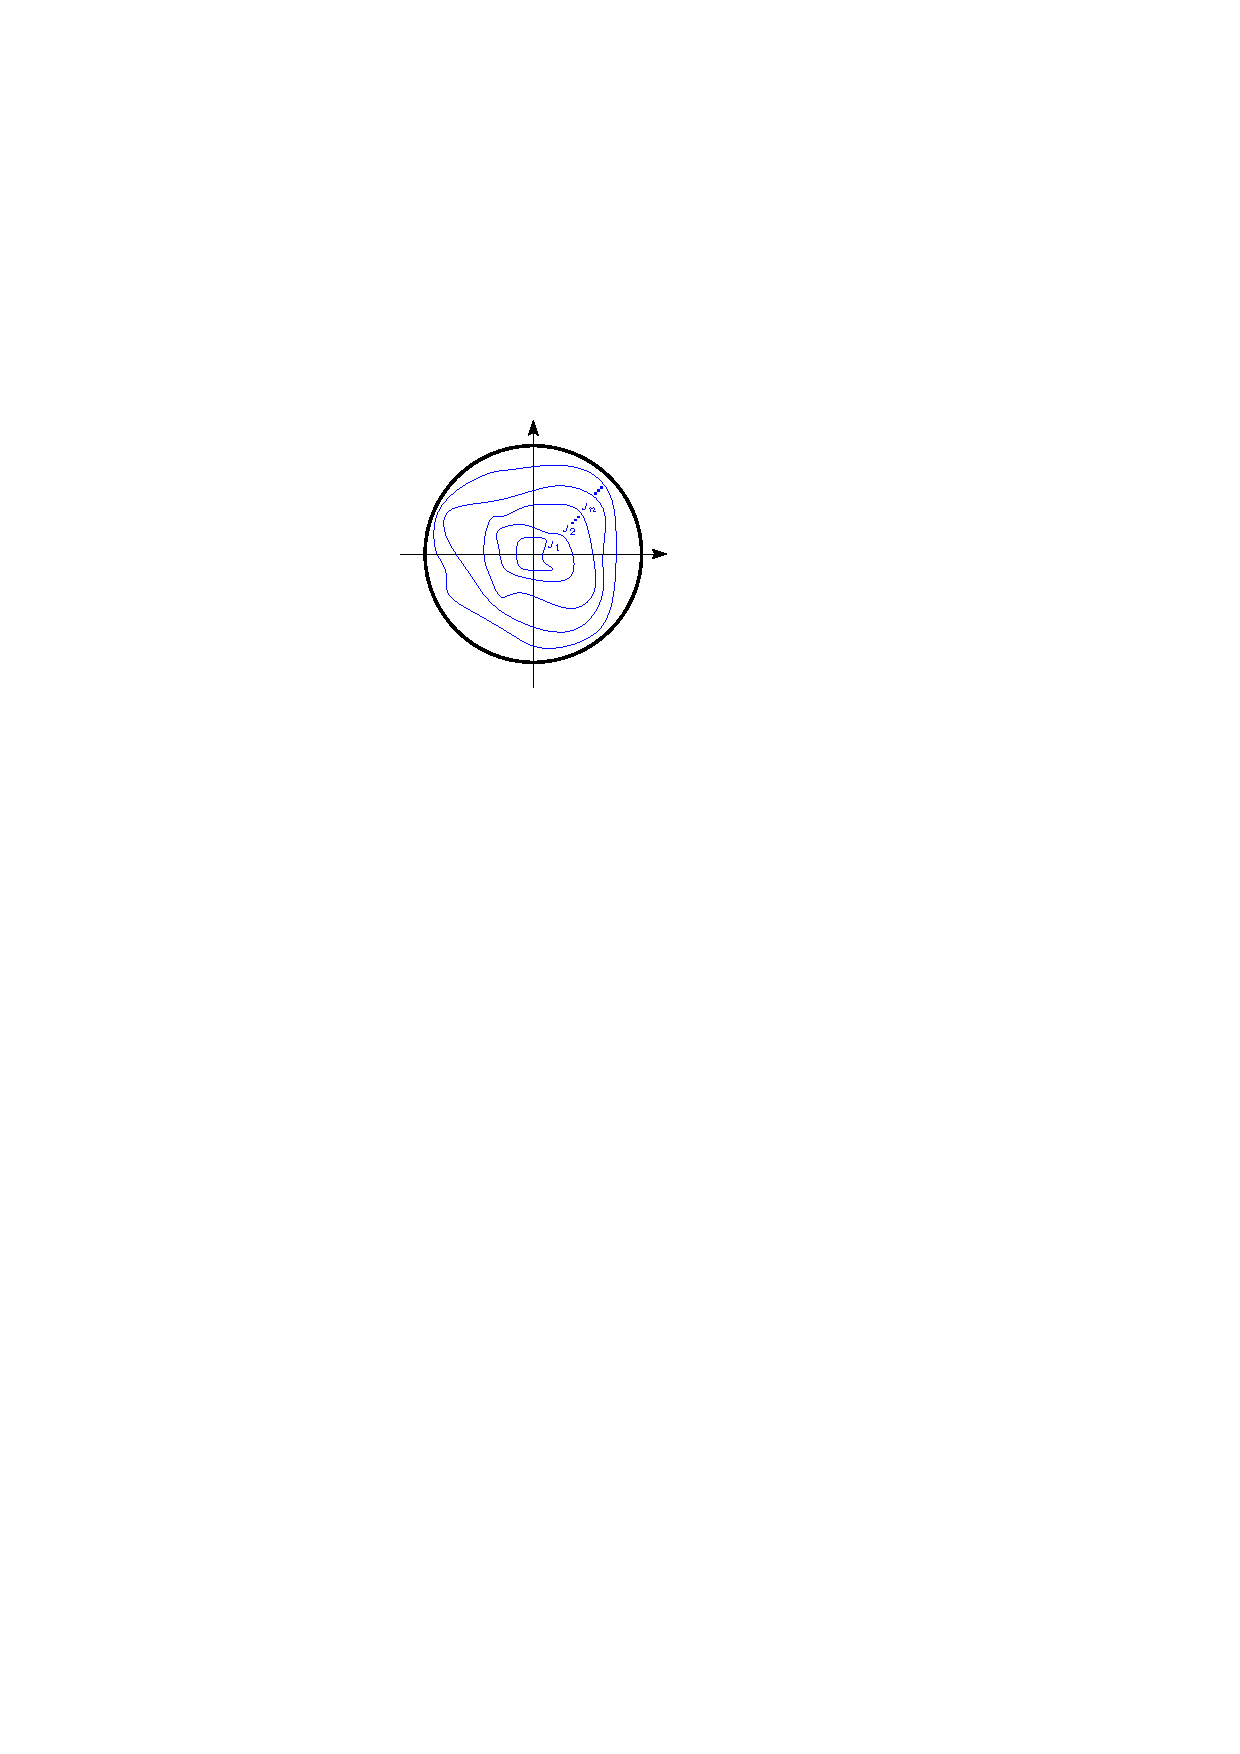
\includegraphics[width=0.2\textwidth, page=1]{pics.pdf}
\hspace*{0.5in}
\includegraphics[width=0.2\textwidth, page=2]{pics.pdf}
\end{center}

Now, pick a number at random between 0 and 1 and write it in its binary decimal form.

Examples: $\frac{1}{4} = 0.01000000 \ldots; \; \frac{1}{3} = 0.01010101 \ldots$

Associate that number with an infinite series of the form $\Sigma \pm z^n$, where the plus or minus signs are determined by the
corresponding digits in the binary expansion of the number chosen: $0 \longrightarrow +; \; 1 \longrightarrow 1$.

Examples:

$\frac{1}{4} = 0.01000000 \ldots $ gives \; $\Sigma \pm z^n = 1-z+z^2+z^3+z^4+z^5+z^6+z^7 + \cdots $;

$\frac{1}{3} = 0.01010101 \ldots$ gives \; $\Sigma\pm z^n = 1-z+z^2-z^3+z^4-z^5+z^6-z^7 + \cdots $.

\item \textbf{The Project}

What is the probability that the number picked results in an infinite series that is strongly annular? In the \emph{Monthly} article we
proved that the probability is either zero or one (independently of the zero-one law), and also found uncountable collections of
numbers giving rise to series that have and do not have that property. So, what is the probability---zero or one?

\item \textbf{Contact Details}

Russell W.\ Howell is Kathleen Smith Professor of Mathematics at Westmont College, Santa Barbara, CA, \;
email: \href{mailto:howell@westmont.edu}{howell@westmont.edu}.
\end{enumerate}

\end{document}
